\begin{document}

%% Project-specific Preambles
\settoggle{includelogo}{true}

\newcommand{\thesubject}{Informatik}
\newcommand{\thetopic}{Numerische Berechnungen}
\newcommand{\thelogo}{Logos/FreeFlower.pdf}
\newcommand{\logosize}{.5\textwidth}

\lhead[\leftmark]{\thetopic}
\rhead[\thesubject]{\textcopyleft{} \href{https://github.com/CyrilBlum/FreeFlower}{FreeFlower}, \the\year}

\settoggle{emoji}{false}
\def\arrayB{"grinning-face","bar-chart","laptop","technologist","robot","woman-student","hundred-points"}
\maketitlepage{\thetopic}{}
\tableofcontents
\newpage

%% Inhalt
\chapter{Quadraturregeln}\label{ch:quadraturregeln}

Wie gross ist die Fläche zwischen einem Funktionsgraphen und der $x$-Achse?
Bei einem Rechteck genügt es, Breite und Höhe zu multiplizieren. Bei einer gekrümmten Begrenzung ist das weniger einfach.
\tib{Quadraturregeln} sind Verfahren, mit denen wir solche Flächeninhalte näherungsweise berechnen. Dazu ersetzen wir die gesuchte Fläche beispielsweise durch Rechtecke oder Trapeze, deren Flächeninhalte sich leicht berechnen lassen.

\section{Grundidee und Parameter}

Wir betrachten eine Funktion $f$, deren Graph im Bereich von $a$ bis $b$ ohne Sprünge verläuft. Dabei gilt $a<b$. In diesem Kapitel setzen wir voraus, dass der Graph auf oder oberhalb der $x$-Achse liegt, also $f(x)\geq 0$ gilt.
Gesucht ist der Flächeninhalt $A$ zwischen dem Graphen, der $x$-Achse und den beiden senkrechten Grenzen bei $x=a$ und $x=b$.

Für die ersten drei Verfahren teilen wir das Intervall in $n$ gleich breite Teilintervalle. Dabei muss $n$ eine positive ganze Zahl sein. Die Breite $h$ und die Intervallgrenzen $x_i$ lauten:
\[
    h = \frac{b-a}{n}, \qquad x_i = a + i\cdot h \quad (i=0,\ldots,n).
\]
Das Teilintervall mit dem Index $i$ reicht somit von $x_i$ bis $x_{i+1}$. In Python durchläuft \lstinline|range(n)| die Indizes $0$ bis $n-1$.

Die Funktionen in den folgenden Listings erhalten vier Argumente:
\begin{itemize}
    \item \lstinline|f|: die Funktion, unter deren Graphen wir den Flächeninhalt näherungsweise berechnen.
    \item \lstinline|a| und \lstinline|b|: die linke und rechte Grenze des Intervalls.
    \item \lstinline|n|: die Anzahl der Teilintervalle.
\end{itemize}
Die Variable \lstinline|breite| entspricht $h$. In \lstinline|summe| werden die Beiträge der einzelnen Teilintervalle addiert. Die Implementierungen setzen gültige Argumente voraus und prüfen diese nicht selbst.

\begin{myremark}
Die folgende interaktive Visualisierung zeigt, wie Rechtecke und Trapeze die Fläche unter einem Funktionsgraphen annähern:
\begin{center}
    \url{https://anchlopecki.github.io/AI_Visualizers/riemann_sum.html}
\end{center}
Funktion, Intervallgrenzen und Anzahl der Teilintervalle lassen sich verändern. Die Einstellungen \enquote{Left}, \enquote{Midpoint} und \enquote{Trapezoid} entsprechen der linken Riemannsumme, der Mittelpunktsregel und der Trapezregel, die wir im Folgenden kennenlernen.
\end{myremark}

\section{Linke Riemannsumme}

Bei der \tib{linken Riemannsumme} ersetzen wir die Fläche in jedem Teilintervall durch ein Rechteck. Als Höhe verwenden wir den Funktionswert am \textbf{linken Endpunkt} $x_i$:
\[
    L_n = h\sum_{i=0}^{n-1} f(x_i).
\]
Wenn die Funktionswerte von links nach rechts nur zunehmen oder gleich bleiben, unterschätzt die linke Riemannsumme den gesuchten Flächeninhalt. Wenn sie nur abnehmen oder gleich bleiben, überschätzt sie ihn. Bei einer konstanten Funktion stimmt die Näherung genau.

\begin{lstlisting}[language=Python, caption={Linke Riemannsumme}, label={lst:quadratur-links}]
def linke_riemannsumme(f, a, b, n):
    summe = 0
    breite = (b - a) / n

    # Summiere die Flächeninhalte der n Rechtecke:
    for i in range(n):
        # Linker Endpunkt des Rechtecks
        x = a + i * breite
        hoehe = f(x)

        summe += breite * hoehe

    return summe
\end{lstlisting}

\section{Mittelpunktsregel}

Auch die \tib{Mittelpunktsregel} verwendet Rechtecke. Die Höhe wird jedoch in der \textbf{Mitte des Teilintervalls} bestimmt:
\[
    M_n = h\sum_{i=0}^{n-1} f\left(x_i+\frac{h}{2}\right).
\]
Bei einer linearen Funktion gleichen sich die zu viel und die zu wenig gezählten Flächen innerhalb eines Teilintervalls genau aus. Deshalb liefert die Mittelpunktsregel für lineare Funktionen bereits den exakten Flächeninhalt, abgesehen von möglichen Rundungsfehlern im Computer.

\begin{myexercise}[Mittelpunktsregel implementieren]\label{ex:quadratur-mittelpunktsregel}
Verwenden Sie die linke Riemannsumme aus \cref{lst:quadratur-links} als Vorbild.
\begin{aenum}
    \item Ergänzen Sie im folgenden Codegerüst die mit \lstinline|...| markierten Stellen. Berechnen Sie für jedes Teilintervall dessen Mittelpunkt, die Höhe des Rechtecks und seinen Beitrag zur Gesamtfläche.
    \item Testen Sie Ihre Funktion mit $f(x)=x^2$, $a=0$, $b=1$ und $n=4$. Vergleichen Sie das Ergebnis mit der linken Riemannsumme und dem tatsächlichen Flächeninhalt $A=1/3$ (siehe \cref{ex:quadratur-quadratfunktion}). Welche Näherung liegt näher am tatsächlichen Wert?
    \item Testen Sie zusätzlich $g(x)=x+1$ auf $[1,3]$ mit $n=4$. Die Fläche ist ein Trapez mit der Breite $2$ und den Höhen $2$ und $4$. Welches Ergebnis erwarten Sie? Prüfen Sie, ob Ihre Funktion dieses liefert.
\end{aenum}
Die Platzhalter müssen vor dem Ausführen durch passende Python-Ausdrücke ersetzt werden.

\begin{lstlisting}[language=Python, caption={Codegerüst zur Mittelpunktsregel}]
def mittelpunktsregel(f, a, b, n):
    summe = 0
    breite = (b - a) / n

    for i in range(n):
        links = a + i * breite
        mitte = ...
        hoehe = ...
        summe += ...

    return summe


def f(x):
    return x**2


print(mittelpunktsregel(f, 0, 1, 4))
\end{lstlisting}

\begin{myanswer}
\begin{lstlisting}[language=Python, caption={Musterlösung zur Mittelpunktsregel}, label={lst:quadratur-mitte}]
def mittelpunktsregel(f, a, b, n):
    summe = 0
    breite = (b - a) / n

    # Summiere die Flächeninhalte der n Rechtecke:
    for i in range(n):
        mitte = (a + i * breite) + 0.5 * breite
        hoehe = f(mitte)
        summe += breite * hoehe

    return summe
\end{lstlisting}

Für $f(x)=x^2$ ergibt sich $M_4=0.328125$. Dieser Wert liegt näher an $1/3$ als die linke Riemannsumme $L_4=0.21875$. Beide Näherungen sind hier zu klein.

Für den zweiten Test ergänzen wir:
\begin{lstlisting}[language=Python]
def g(x):
    return x + 1


print(mittelpunktsregel(g, 1, 3, 4))
\end{lstlisting}
Der erwartete Flächeninhalt ist $A=2\cdot(2+4)/2=6$. Die Ausgabe ist \lstinline|6.0|. Die Mittelpunktsregel liefert für diese lineare Funktion den exakten Wert. Zugleich prüft dieser Test ein Intervall, das nicht bei $0$ beginnt.
\end{myanswer}
\end{myexercise}

\section{Trapezregel}

Bei der \tib{Trapezregel} verbinden wir die Funktionswerte an den beiden Endpunkten eines Teilintervalls durch eine gerade Strecke. Für eine nichtnegative Funktion entsteht unter dieser Strecke ein Trapez. Sein Flächeninhalt ist die Breite multipliziert mit dem Mittelwert der beiden Höhen:
\[
    T_n = h\sum_{i=0}^{n-1}\frac{f(x_i)+f(x_{i+1})}{2}.
\]
Auch die Trapezregel ist für lineare Funktionen exakt, abgesehen von möglichen Rundungsfehlern.

\begin{myexercise}[Trapezregel implementieren]\label{ex:quadratur-trapezregel}
Entwickeln Sie nun aus der linken Riemannsumme eine Funktion für die Trapezregel.
\begin{aenum}
    \item Ergänzen Sie das Codegerüst. Bestimmen Sie den rechten Endpunkt des Teilintervalls und speichern Sie den Mittelwert der beiden Funktionswerte in \lstinline|m|. Addieren Sie anschliessend den Flächeninhalt des Trapezes zu \lstinline|summe|.
    \item Testen Sie Ihre Funktion wieder mit $f(x)=x^2$, $a=0$, $b=1$ und $n=4$. Vergleichen Sie das Ergebnis mit $A=1/3$ und mit Ihrer Mittelpunktsregel. Welche Näherung ist zu klein, welche zu gross?
    \item Prüfen Sie Ihre Funktion auch mit $g(x)=x+1$ auf $[1,3]$ und $n=4$. Begründen Sie, weshalb die Trapezregel hier den exakten Flächeninhalt liefern sollte.
\end{aenum}

\begin{lstlisting}[language=Python, caption={Codegerüst zur Trapezregel}]
def trapezregel(f, a, b, n):
    summe = 0
    breite = (b - a) / n

    for i in range(n):
        links = a + i * breite
        rechts = ...
        m = ...
        summe += ...

    return summe


def f(x):
    return x**2


print(trapezregel(f, 0, 1, 4))
\end{lstlisting}

\begin{myanswer}
\begin{lstlisting}[language=Python, caption={Musterlösung zur Trapezregel}, label={lst:quadratur-trapez}]
def trapezregel(f, a, b, n):
    summe = 0
    breite = (b - a) / n

    # Summiere die Flächeninhalte der n Trapeze:
    for i in range(n):
        links = a + i * breite
        rechts = (a + i * breite) + breite
        m = (f(links) + f(rechts)) / 2
        summe += breite * m

    return summe
\end{lstlisting}

Für $f(x)=x^2$ ergibt sich $T_4=0.34375$. Die Trapezregel überschätzt hier den tatsächlichen Flächeninhalt $1/3$, während die Mittelpunktsregel mit $M_4=0.328125$ darunter liegt.

\begin{lstlisting}[language=Python]
def g(x):
    return x + 1


print(trapezregel(g, 1, 3, 4))
\end{lstlisting}
Die Ausgabe ist \lstinline|6.0|. Der Graph von $g$ ist eine Gerade. Daher stimmen die geraden Oberkanten der Trapeze genau mit dem Graphen überein. Ihre Flächen ergeben zusammen den tatsächlichen Flächeninhalt $A=6$.
\end{myanswer}
\end{myexercise}

\section{Monte-Carlo-Methode}

\tib{Monte-Carlo-Methoden} verwenden Zufallsstichproben, um eine gesuchte Grösse zu schätzen. Für Flächen betrachten wir zwei Varianten: Wir können Funktionswerte an zufällig gewählten Stellen mitteln oder zufällige Punkte erzeugen und Treffer zählen.

\subsection{Funktionswerte an zufälligen Stellen mitteln}

Die Grundidee lautet: \textbf{Flächeninhalt = Intervallbreite mal mittlere Höhe}. Bei der Mittelpunktsregel haben wir Höhen an regelmässig verteilten Stellen verwendet. Nun wählen wir stattdessen $n$ Stellen $X_1,\ldots,X_n$ unabhängig und gleichverteilt aus $[a,b]$. Gleichverteilt bedeutet, dass gleich breite Teilintervalle dieselbe Chance haben, eine gezogene Stelle zu enthalten. Wir teilen das Intervall dabei nicht in feste Teilintervalle ein.

An jeder gezogenen Stelle berechnen wir die Höhe $f(X_i)$. Der arithmetische Mittelwert dieser Höhen schätzt die mittlere Höhe des Graphen über dem gesamten Intervall:
\[
    \overline{H}=\frac{1}{n}\sum_{i=1}^{n}f(X_i),
    \qquad A\approx (b-a)\cdot\overline{H}.
\]
Anschaulich ersetzen wir die gesuchte Fläche durch ein einziges Rechteck mit der Breite $b-a$ und der geschätzten mittleren Höhe $\overline{H}$. Wir benötigen dafür nur zufällige $x$-Koordinaten, keine zufälligen $y$-Koordinaten.

\begin{lstlisting}[language=Python, caption={Monte Carlo durch Mittelung zufälliger Höhen}, label={lst:quadratur-monte-carlo-mittelwert}]
import random


def monte_carlo_mittelwert(f, a, b, n):
    summe = 0

    for i in range(n):
        x = random.uniform(a, b)
        summe += f(x)

    mittlere_hoehe = summe / n
    return (b - a) * mittlere_hoehe
\end{lstlisting}

Die Funktion setzt $a<b$, eine positive ganze Zahl $n$ und eine stetige, nichtnegative Funktion $f$ auf $[a,b]$ voraus. Eine obere Grenze für die Funktionswerte müssen wir nicht kennen. Auf dem Einheitsintervall $[0,1]$ ist die Breite $1$, sodass der Mittelwert allein bereits die Fläche schätzt. Auf anderen Intervallen darf der Faktor $b-a$ nicht fehlen: Für die konstante Höhe $f(x)=3$ auf $[1,3]$ ist beispielsweise die mittlere Höhe $3$, der Flächeninhalt aber $2\cdot 3=6$.

\subsection{Treffer in einem umgebenden Rechteck zählen}

Eine zweite Variante erzeugt zufällige Punkte in einem Rechteck, das die gesuchte Fläche vollständig enthält. Der Anteil der Punkte unterhalb des Graphen schätzt den Flächenanteil am Rechteck. Wir betrachten hier das Einheitsquadrat.

\begin{myattention}
Die folgende Implementierung ist auf das Intervall $[0,1]$ beschränkt und setzt $0\leq f(x)\leq 1$ für alle $x$ in diesem Intervall voraus. Die gesuchte Fläche liegt somit vollständig im Einheitsquadrat. Ausserdem muss \lstinline|n| eine positive ganze Zahl sein. Hier bezeichnet sie die Anzahl der zufälligen Punkte.
\end{myattention}

Wir wählen beide Koordinaten eines Punktes unabhängig und gleichverteilt zwischen $0$ und $1$. Ein Punkt $(p_x,p_y)$ gilt als Treffer, wenn $p_y\leq f(p_x)$ ist. Der Anteil der Treffer schätzt den Anteil der gesuchten Fläche am Einheitsquadrat. Da dieses den Flächeninhalt $1$ hat, gilt:
\[
    A \approx \frac{\text{Anzahl Treffer}}{n}.
\]

\begin{lstlisting}[language=Python, caption={Monte-Carlo-Methode im Einheitsquadrat}, label={lst:quadratur-monte-carlo}]
import random


def monte_carlo(f, n):
    treffer = 0

    for i in range(n):
        px = random.uniform(0, 1)
        py = random.uniform(0, 1)
        # P = (px, py) ist ein Punkt im Einheitsquadrat

        if py <= f(px):
            # P liegt unter oder auf dem Funktionsgraphen
            treffer += 1

    return treffer / n
\end{lstlisting}

Auch das Trefferzählen ist eine Mittelung: Ein Treffer erhält den Wert $1$, ein anderer Punkt den Wert $0$. Der Mittelwert dieser Werte ist genau der Trefferanteil. Bei der ersten Variante geht dagegen jede ausgewertete Höhe direkt in den Mittelwert ein. Sie nutzt damit mehr Information als die blosse Entscheidung \enquote{Treffer oder kein Treffer} und hat unter den hier betrachteten Voraussetzungen bei gleicher Stichprobenzahl höchstens gleich grosse zufällige Schwankungen.

Anders als die ersten drei Verfahren liefern beide Monte-Carlo-Varianten bei wiederholter Ausführung im Allgemeinen unterschiedliche Ergebnisse. Mehr Stichproben verringern die typischen zufälligen Abweichungen, garantieren aber nicht bei jedem einzelnen Durchlauf ein genaueres Ergebnis.

\section{Anwendung und Vergleich}

\begin{myexample}\label{ex:quadratur-quadratfunktion}
Wir betrachten die Fläche unter dem Graphen von $f(x)=x^2$ zwischen $x=0$ und $x=1$. Als Vergleichswert verwenden wir den exakten Flächeninhalt
\[
    A = \frac{1}{3}.
\]
Die Herleitung dieses exakten Werts behandeln wir hier nicht. Wir untersuchen, wie nahe unsere Näherungen an diesen Wert herankommen.
Mit $n=4$ Teilintervallen und der Breite $h=0.25$ ergeben sich folgende Näherungen:
\begin{center}
    \begin{tabular}{lrl}
        \toprule
        Verfahren & Näherungswert & Vergleich mit $1/3$ \\
        \midrule
        Linke Riemannsumme & $0.21875$ & zu klein \\
        Mittelpunktsregel & $0.328125$ & zu klein \\
        Trapezregel & $0.34375$ & zu gross \\
        \bottomrule
    \end{tabular}
\end{center}
Beispielsweise verwendet die linke Riemannsumme die Höhen an den Stellen $0$, $0.25$, $0.5$ und $0.75$:
\[
    L_4 = 0.25\cdot\left(0^2+0.25^2+0.5^2+0.75^2\right)=0.21875.
\]
\end{myexample}

Nachdem Sie Ihre eigenen Implementierungen und die beiden Monte-Carlo-Funktionen in derselben Python-Datei eingefügt haben, können Sie die Verfahren wie folgt aufrufen:

\begin{lstlisting}[language=Python, caption={Anwendung auf die Funktion f(x) = x**2}, label={lst:quadratur-anwendung}]
def f(x):
    return x**2


print(trapezregel(f, 0, 1, 1000))
print(monte_carlo_mittelwert(f, 0, 1, 1000))
print(monte_carlo(f, 1000))
\end{lstlisting}

Dabei übergeben wir mit \lstinline|f| die Funktion selbst. Erst innerhalb des jeweiligen Verfahrens wird sie für die benötigten Stellen ausgewertet.
Die Trapezregel liefert hier ungefähr $0.3333335$. Die Ergebnisse beider Monte-Carlo-Varianten schwanken zufällig um $1/3$. Feste Ausgaben lassen sich dafür nicht angeben.

\begin{mysummary}[Genauigkeit und Rechenaufwand]
Bei den ersten drei Verfahren bedeutet ein grösseres $n$ schmalere Teilintervalle und mehr Rechenarbeit. Für die hier betrachteten Funktionen nähern sich ihre Ergebnisse mit wachsendem $n$ dem tatsächlichen Flächeninhalt an, wenn wir Rundungsfehler ausser Acht lassen.
Die Mittelpunktsregel und die Trapezregel sind bei hinreichend glatten Funktionen typischerweise genauer als die linke Riemannsumme bei gleicher Anzahl Teilintervalle.
Bei den Monte-Carlo-Varianten erhöht ein grösseres $n$ die Anzahl der zufällig gewählten Stellen beziehungsweise Punkte. Für die Fläche unter der hier betrachteten Parabel sind die Mittelpunktsregel und die Trapezregel in der Regel effizienter.
\end{mysummary}

\section{Fläche zwischen zwei Graphen}

\begin{myexercise}[Zwei Graphen kreuzen sich mehrfach]\label{ex:quadratur-zwischen-graphen}
Gegeben sind die beiden Funktionen
\[
    f(x)=0.5+0.4\sin(4\pi x), \qquad
    g(x)=0.5+0.4\cos(4\pi x)
\]
auf dem Intervall $[0,1]$. Die Winkel werden im Bogenmass angegeben.
Gesucht ist der gesamte Flächeninhalt zwischen den beiden Graphen, begrenzt durch $x=0$ und $x=1$.
Alle schattierten Teilflächen zählen positiv, auch wenn die Graphen ihre Reihenfolge wechseln.

\begin{center}
    % TikZ verwendet Grad; 4*pi*x im Bogenmass entspricht 720*x Grad.
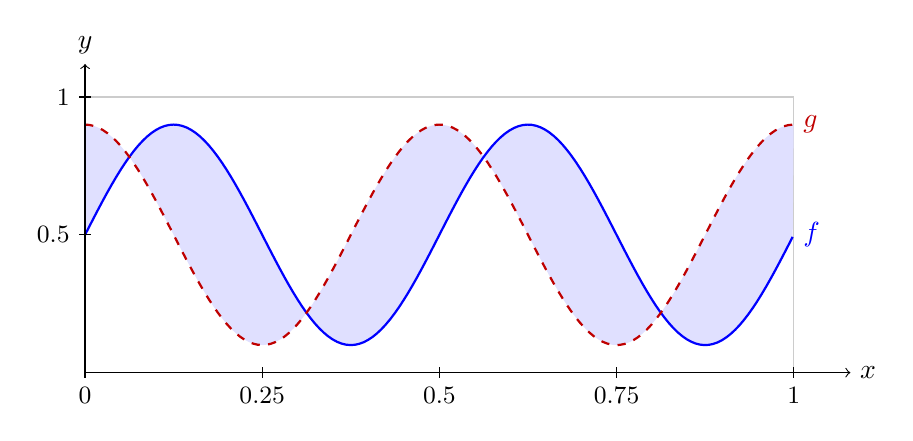
\begin{tikzpicture}[x=9cm, y=3.5cm]
    \draw[gray!40] (0,0) rectangle (1,1);
    \path[fill=blue!12]
        plot[domain=0:1, samples=161] (\x,{0.5+0.4*sin(720*\x)})
        -- plot[domain=1:0, samples=161] (\x,{0.5+0.4*cos(720*\x)})
        -- cycle;
    \draw[blue, thick] plot[domain=0:1, samples=161]
        (\x,{0.5+0.4*sin(720*\x)});
    \draw[red!75!black, thick, dashed] plot[domain=0:1, samples=161]
        (\x,{0.5+0.4*cos(720*\x)});
    \draw[->] (0,0) -- (1.08,0) node[right] {$x$};
    \draw[->] (0,0) -- (0,1.12) node[above] {$y$};
    \foreach \x in {0,0.25,0.5,0.75,1}
        \draw (\x,0.02) -- (\x,-0.02) node[below] {\small $\x$};
    \foreach \y in {0.5,1}
        \draw (0.008,\y) -- (-0.008,\y) node[left] {\small $\y$};
    \node[blue, right] at (1,0.5) {$f$};
    \node[red!75!black, right] at (1,0.9) {$g$};
\end{tikzpicture}

\end{center}

\begin{aenum}
    \item Begründen Sie, weshalb beide Graphen vollständig im Einheitsquadrat liegen. Beschreiben Sie eine Bedingung, die prüft, ob ein Punkt $(p_x,p_y)$ zwischen den Graphen liegt, unabhängig davon, welcher Graph gerade oben liegt.
    \item \textbf{Monte Carlo:} Schreiben Sie eine Funktion \lstinline|monte_carlo_zwischen(f, g, n)|. Passen Sie dazu \cref{lst:quadratur-monte-carlo} so an, dass nur Punkte zwischen den beiden Graphen als Treffer zählen. Alternativ können Sie nur zufällige $x$-Koordinaten wählen und die senkrechten Abstände zwischen den Graphen mitteln (vgl.\ \cref{lst:quadratur-monte-carlo-mittelwert}). Führen Sie mit Ihrer gewählten Variante für $n=1000$, $n=10000$ und $n=100000$ jeweils fünf Durchläufe aus und notieren Sie die Ergebnisse.
    \item \textbf{Trapezregel:} Definieren Sie eine Hilfsfunktion \lstinline|abstand(x)|, die den senkrechten Abstand zwischen den Graphen liefert. Verwenden Sie dafür \lstinline|abs| und wenden Sie Ihre Trapezregel aus \cref{ex:quadratur-trapezregel} auf diese Funktion an. Berechnen Sie Näherungen für $n=10$, $n=100$ und $n=1000$ Teilintervalle.
    \item Vergleichen Sie beide Verfahren mit dem Referenzwert $A\approx 0.3601265265$. Berechnen Sie jeweils die absolute Abweichung. Weshalb wäre es falsch, zuerst die beiden Flächen unter $f$ und $g$ zu berechnen und anschliessend den Betrag ihrer Differenz zu nehmen? Erklären Sie auch, weshalb ein grösseres $n$ bei Monte Carlo nicht in jedem Durchlauf ein genaueres Ergebnis garantiert.
\end{aenum}

Die Funktionen können Sie in Python wie folgt definieren:
\begin{lstlisting}[language=Python]
import math


def f(x):
    return 0.5 + 0.4 * math.sin(4 * math.pi * x)


def g(x):
    return 0.5 + 0.4 * math.cos(4 * math.pi * x)
\end{lstlisting}

% Die lange Lösung bleibt ohne innere Box über mehrere Seiten umbrechbar.
\begin{myanswer}[ex:quadratur-zwischen-graphen]
Sinus und Kosinus liegen zwischen $-1$ und $1$. Daher liegen die Funktionswerte beider Funktionen zwischen $0.1$ und $0.9$ und somit innerhalb des Einheitsquadrats.
Die gesuchte Trefferbedingung lautet
\[
    \min(f(p_x),g(p_x))\leq p_y\leq\max(f(p_x),g(p_x)).
\]
\textbf{Monte Carlo durch Trefferzählen:}\\
Da das umgebende Quadrat den Flächeninhalt $1$ hat, genügt der Anteil der Treffer als Schätzung.

\begin{lstlisting}[language=Python, caption={Monte Carlo für die Fläche zwischen zwei Graphen}]
import random


def monte_carlo_zwischen(f, g, n):
    treffer = 0

    for i in range(n):
        px = random.uniform(0, 1)
        py = random.uniform(0, 1)
        fx = f(px)
        gx = g(px)

        # Die Reihenfolge der Graphen kann wechseln.
        if min(fx, gx) <= py <= max(fx, gx):
            treffer += 1

    return treffer / n


referenz = 0.8 * math.sqrt(2) / math.pi
for n in (1000, 10000, 100000):
    for durchlauf in range(5):
        a = monte_carlo_zwischen(f, g, n)
        print(n, durchlauf + 1, a, abs(a - referenz))
\end{lstlisting}

Für die Trapezregel ist die Höhe an jeder Stelle der \textbf{Betrag der Differenz} der Funktionswerte. Wir verwenden die bestehende Funktion \lstinline|trapezregel|:
\begin{lstlisting}[language=Python, caption={Trapezregel für den Abstand der Graphen}]
def abstand(x):
    return abs(f(x) - g(x))


for n in (10, 100, 1000):
    a = trapezregel(abstand, 0, 1, n)
    print(n, a, abs(a - referenz))
\end{lstlisting}

Die Trapezregel liefert folgende gerundete Werte:
\begin{center}
    \begin{tabular}{rrr}
        \toprule
        Teilintervalle $n$ & Näherungswert & Absolute Abweichung \\
        \midrule
        $10$ & $0.3616117617$ & $0.0014852352$ \\
        $100$ & $0.3601857717$ & $0.0000592453$ \\
        $1000$ & $0.3601288960$ & $0.0000023695$ \\
        \bottomrule
    \end{tabular}
\end{center}
Der exakte Vergleichswert ist $A=0.8\sqrt{2}/\pi$. Seine Herleitung mit Integralrechnung ist für diese Aufgabe nicht erforderlich.

\textbf{Alternative Monte-Carlo-Lösung: Abstände mitteln}\\
Wir wählen nur die Stellen $X_i$ unabhängig und gleichverteilt aus $[0,1]$ und berechnen dort jeweils den senkrechten Abstand $|f(X_i)-g(X_i)|$. Der Mittelwert dieser Abstände schätzt die mittlere Höhe der gesuchten Fläche. Da die Intervallbreite $1$ ist, gilt:
\[
    A\approx\frac{1}{n}\sum_{i=1}^{n}|f(X_i)-g(X_i)|.
\]
Durch den Betrag werden alle Teilflächen positiv gezählt, unabhängig davon, wie oft sich die Graphen kreuzen. Die Schnittpunkte müssen wir nicht vorher bestimmen.

\begin{lstlisting}[language=Python, caption={Alternative: zufällige Abstände mitteln}]
def monte_carlo_zwischen_mittelwert(f, g, n):
    summe = 0

    for i in range(n):
        x = random.uniform(0, 1)
        summe += abs(f(x) - g(x))

    return summe / n


for n in (1000, 10000, 100000):
    for durchlauf in range(5):
        a = monte_carlo_zwischen_mittelwert(f, g, n)
        print(n, durchlauf + 1, a, abs(a - referenz))
\end{lstlisting}

Mit der bereits definierten Funktion \lstinline|abstand| können wir stattdessen auch direkt die allgemeine Mittelungsfunktion verwenden:
\begin{lstlisting}[language=Python]
a = monte_carlo_mittelwert(abstand, 0, 1, n)
\end{lstlisting}
Auf einem allgemeinen Intervall $[a,b]$ werden die Stellen dort gezogen und der mittlere Abstand zusätzlich mit $b-a$ multipliziert. Bei dieser Aufgabe schwankt die Mittelungsvariante bei gleicher Stichprobenzahl weniger stark als das Trefferzählen. Ein einzelner Durchlauf kann trotzdem ungenauer ausfallen.

Die Flächen unter $f$ und $g$ sind hier beide $0.5$: Sinus und Kosinus durchlaufen jeweils zwei vollständige Perioden, sodass sich ihre positiven und negativen Beiträge zur Grundhöhe $0.5$ aufheben. Die Differenz der beiden Flächen ist deshalb $0$, obwohl die Fläche zwischen den Graphen positiv ist. Der Betrag muss \emph{vor} dem Aufsummieren an jeder Stelle gebildet werden.

Die Monte-Carlo-Ergebnisse schwanken zufällig um den Referenzwert. Bei grösserem $n$ werden die typischen Abweichungen kleiner. Einzelne Durchläufe können trotzdem weiter vom Referenzwert entfernt liegen. Die Trapezregel liefert bei gleichem $n$ stets dasselbe Ergebnis und erreicht bei dieser Aufgabe bereits mit wenigen Auswertungen eine hohe Genauigkeit. Dabei bezeichnet $n$ bei Monte Carlo die Anzahl der zufällig gewählten Stellen beziehungsweise Punkte, bei der Trapezregel die Anzahl der Teilintervalle.
\end{myanswer}
\end{myexercise}


\end{document}
